\documentclass[aspectratio=169,10pt]{beamer}

% ---------------------------------------------------------------------------
% Packages
% ---------------------------------------------------------------------------
\usepackage[T5]{fontenc}
\usepackage[utf8]{inputenc}
\usepackage{lmodern}
\usepackage{booktabs}
\usepackage{tabularx}
\usepackage{colortbl}
\usepackage{tikz}
\usetikzlibrary{arrows.meta,calc,positioning,shapes.geometric,fit,backgrounds}
\usepackage{graphicx}
\usepackage{amsmath}

% ---------------------------------------------------------------------------
% Palette (minimalist academic, HCMUS blue)
% ---------------------------------------------------------------------------
\definecolor{HCMUSBlue}{HTML}{165A9F}
\definecolor{DarkNavy}{HTML}{0D2E52}
\definecolor{Ink}{HTML}{1A1A1A}
\definecolor{Slate}{HTML}{5B6570}
\definecolor{SoftBg}{HTML}{F4F7FA}
\definecolor{LineGray}{HTML}{D8DEE6}
\definecolor{L1Blue}{HTML}{165A9F}
\definecolor{L2Orange}{HTML}{C2560F}
\definecolor{L3Aqua}{HTML}{0E8A6A}
\definecolor{WarnRed}{HTML}{B3261E}
\definecolor{GoldAmber}{HTML}{B7791F}

% ---------------------------------------------------------------------------
% Theme: quiet, information-first (no busy headers)
% ---------------------------------------------------------------------------
\usetheme{default}
\setbeamercolor{normal text}{fg=Ink,bg=white}
\setbeamercolor{structure}{fg=HCMUSBlue}
\setbeamercolor{frametitle}{fg=DarkNavy,bg=white}
\setbeamercolor{title}{fg=DarkNavy}
\setbeamercolor{subtitle}{fg=Slate}
\setbeamercolor{item}{fg=HCMUSBlue}
\setbeamercolor{itemize item}{fg=HCMUSBlue}
\setbeamercolor{enumerate item}{fg=HCMUSBlue}
\setbeamercolor{description item}{fg=DarkNavy}
\setbeamercolor{block title}{fg=white,bg=HCMUSBlue}
\setbeamercolor{block body}{fg=Ink,bg=SoftBg}
\setbeamercolor{block title alerted}{fg=white,bg=WarnRed}
\setbeamercolor{block body alerted}{fg=Ink,bg=SoftBg}
\setbeamercolor{block title example}{fg=white,bg=L3Aqua}
\setbeamercolor{block body example}{fg=Ink,bg=SoftBg}
\setbeamercolor{footnote}{fg=Slate}
\setbeamercolor{footnote mark}{fg=HCMUSBlue}

\setbeamertemplate{navigation symbols}{}
\setbeamertemplate{itemize item}{\raisebox{0.35ex}{\scriptsize$\blacktriangleright$}}
\setbeamertemplate{itemize subitem}{\raisebox{0.35ex}{\scriptsize$\circ$}}
\setbeamertemplate{enumerate item}{\insertenumlabel.}
\setbeamertemplate{blocks}[rounded][shadow=false]

% Frametitle: title + thin rule
\setbeamertemplate{frametitle}{%
  \vspace{0.15cm}%
  \begin{beamercolorbox}[wd=\textwidth,sep=0pt]{frametitle}%
    \insertframetitle\strut
    \vspace{-0.15cm}
    {\color{HCMUSBlue}\rule{\textwidth}{1.2pt}}
  \end{beamercolorbox}\vspace{0.25cm}
}

% Footline with reserved height and separate backup numbering.
\newif\ifbackupslides
\backupslidesfalse
\newcounter{backupslide}
\setbeamertemplate{footline}{%
  \leavevmode\hbox{%
    \begin{beamercolorbox}[wd=\paperwidth,ht=2.8ex,dp=1.2ex,left]{normal text}%
      \hspace*{0.4cm}{\scriptsize\color{Slate}Truy hồi đa phương thức có giải thích bằng đồ thị\quad|\quad Nhóm 02\quad|\quad Học máy với dữ liệu đồ thị}%
      \hfill{\scriptsize\ifbackupslides B\arabic{backupslide}/8\else\insertframenumber/\inserttotalframenumber\fi}\hspace*{0.4cm}%
    \end{beamercolorbox}%
  }\vskip3pt%
}

\setbeamertemplate{headline}{}
\setbeamertemplate{caption}[numbered]
\setbeamertemplate{caption label separator}{: }

\newcolumntype{L}[1]{>{\raggedright\arraybackslash}p{#1}}
\newcolumntype{C}[1]{>{\centering\arraybackslash}p{#1}}
\newcolumntype{Y}{>{\raggedright\arraybackslash}X}

% Level tag in frametitle area
\newcommand{\leveltag}[2]{%
  \tikz[baseline=(x.base)]{\node[fill=#1,text=white,inner xsep=5pt,inner ysep=1.5pt,
    rounded corners=2pt,font=\scriptsize\bfseries](x){#2};}\ %
}
\newcommand{\srcref}[1]{\,\textsuperscript{\scriptsize\textcolor{Slate}{[#1]}}}

% ---------------------------------------------------------------------------
\title[Truy vấn Đa phương thức + XAI Đồ thị]{Truy hồi Đa phương thức có Giải thích bằng Đồ thị}
\subtitle{Đồ án 03 --- Học máy với dữ liệu đồ thị --- Nhóm 02}
\author[]{%
  \footnotesize
  Chung Gia Khánh (23120282) \quad Lê Hoàng Mỹ Hạ (23120038) \quad Hàn Vũ Phương Uyên (23120106)\\
  Trần Gia Hiển (23120123) \quad Nguyễn An Nghiệp (23127234)
}
\institute[]{%
  \scriptsize
  Khoa Công nghệ Thông tin, Trường Đại học Khoa học Tự nhiên, ĐHQG-HCM\\
  Cán bộ hướng dẫn: TS. Lê Ngọc Thành \quad ThS. Huỳnh Lâm Hải Đăng
}
\date{Tháng 11 năm 2026}

\begin{document}

% ===========================================================================
% 01 --- Title
% ===========================================================================
\begin{frame}[plain]
  \begin{tikzpicture}[remember picture,overlay]
    \fill[HCMUSBlue] (current page.north west) rectangle ($(current page.north east)+(0,-0.10cm)$);
    \fill[DarkNavy] ($(current page.north west)+(0,-0.10cm)$) rectangle ($(current page.north east)+(0,-0.16cm)$);
    \node[anchor=north west] at ($(current page.north west)+(0.7cm,-0.22cm)$) {
      
\includegraphics[height=0.72cm]{assets/logos/logo_khtn.png}
    };
    \node[anchor=north east, text=white, font=\scriptsize\bfseries] at ($(current page.north east)+(-0.7cm,-0.30cm)$) {
      TRƯỜNG ĐẠI HỌC KHOA HỌC TỰ NHIÊN --- ĐHQG-HCM
    };
    \fill[SoftBg] (current page.south west) rectangle ($(current page.south west)+(16.9cm,2.1cm)$);
    \draw[LineGray, line width=0.6pt] (current page.south west) ++(0,2.1cm) -- ++(16.9cm,0);
  \end{tikzpicture}
  \vspace{1.6cm}
  \begin{center}
    {\Large\bfseries\color{DarkNavy} Truy hồi Đa phương thức có Giải thích bằng Đồ thị}\\[0.45cm]
    {\normalsize\color{HCMUSBlue} Liệu biểu diễn tăng cường đồ thị có cải thiện truy vấn đa phương thức,\\
     và các đóng góp tri thức có thể được định lượng và giải thích xác thực?}\\[0.5cm]
    {\small Đồ án 03 --- Học máy với dữ liệu đồ thị --- Nhóm 02}\\[0.25cm]
    {\footnotesize\color{Slate}
      Chung Gia Khánh (23120282) \;$\cdot$\; Lê Hoàng Mỹ Hạ (23120038) \;$\cdot$\; Hàn Vũ Phương Uyên (23120106) \;$\cdot$\; Trần Gia Hiển (23120123) \;$\cdot$\; Nguyễn An Nghiệp (23127234)}
  \end{center}
  \vspace{0.45cm}
  \begin{center}
    \footnotesize\color{Slate}
    GVHD: TS. Lê Ngọc Thành \quad$\cdot$\quad ThS. Huỳnh Lâm Hải Đăng \quad$\cdot$\quad Tháng 11/2026
  \end{center}
\end{frame}
% ===========================================================================
% 02 --- Research problem
% ===========================================================================
\begin{frame}{CLIP Có Thể Gặp Khó với Truy vấn Quan hệ}
  \begin{columns}[c]
    \begin{column}{0.50\textwidth}
      \begin{block}{Hai giới hạn cần khảo sát}\footnotesize
        \textbf{1. Không suy luận đồ thị tường minh}: CLIP có thể khó phân biệt hai ảnh cùng vật thể nhưng khác \textbf{quan hệ}.\\[0.06cm]
        \textbf{2. Điểm số chưa chỉ ra bằng chứng}: Điểm cosine đơn lẻ không xác định quan hệ nào ảnh hưởng đến kết quả.
      \end{block}
      \vspace{0.08cm}
      \begin{alertblock}{Câu hỏi nghiên cứu}\footnotesize
        Cấu trúc đồ thị có thể cải thiện xếp hạng --- đặc biệt cho các
        truy vấn \textbf{gián tiếp} --- và quan hệ có thể \textbf{định lượng làm bằng chứng giải thích}?
      \end{alertblock}
    \end{column}
    \begin{column}{0.48\textwidth}
      \centering
      \resizebox{\linewidth}{!}{%
      \begin{tikzpicture}[
        img/.style={draw=LineGray, rounded corners=2pt, minimum width=2.1cm, minimum height=1.5cm,
                    fill=SoftBg, align=center, font=\scriptsize},
        lbl/.style={font=\scriptsize\itshape, text=Slate, align=center},
        q/.style={draw=HCMUSBlue, fill=HCMUSBlue, text=white, rounded corners=3pt,
                  align=center, font=\small\bfseries, inner sep=5pt}
      ]
        \node[q] (q) {``a child playing\\football''};
        \node[img, below left=0.55cm and 0.15cm of q] (a) {Ảnh A\\[1pt]
          \textcolor{Slate}{vật thể: child, ball}\\[-1pt]\textcolor{WarnRed}{quan hệ: ?}};
        \node[img, below right=0.55cm and 0.15cm of q] (b) {Ảnh B\\[1pt]
          \textcolor{Slate}{vật thể: child, ball}\\[-1pt]\textcolor{L3Aqua}{quan hệ: plays}};
        \draw[-{Latex[length=2mm]}, HCMUSBlue, thick] (q) -- (a);
        \draw[-{Latex[length=2mm]}, HCMUSBlue, thick] (q) -- (b);
        \node[lbl, below=0.12cm of a] {tương đồng vector:\\khó phân biệt};
        \node[lbl, below=0.12cm of b] {đường đi \texttt{child--plays--football}\\
          liên kết truy vấn đến đúng ảnh};
        \node[font=\scriptsize\itshape, text=Slate, anchor=north west] at (-2.6,-4.35)
          {Ví dụ minh họa (không phải kết quả thực nghiệm)};
      \end{tikzpicture}}
    \end{column}
  \end{columns}
\end{frame}
% ===========================================================================
% 03 --- Objectives / three levels
% ===========================================================================
\begin{frame}{Ba Cấp độ: Mở rộng Từ Cục bộ sang Toàn cục và Giải thích}
  \begin{center}
  \resizebox{\textwidth}{!}{%
  \begin{tikzpicture}[
    box/.style={draw, rounded corners=4pt, inner sep=8pt, align=center, minimum width=4.6cm,
                minimum height=2.5cm, font=\small},
    arrow/.style={-{Latex[length=3mm]}, line width=1.2pt, Slate}
  ]
    \node[box, fill=SoftBg, draw=L1Blue] (l1) {
      \textcolor{L1Blue}{\textbf{Cấp độ 1 --- Tri thức Cục bộ}}\\[0.20cm]
      \footnotesize CLIP đóng băng + GAT cho scene graph\\
      trên Visual Genome\\[0.12cm]
      \scriptsize\textbf{Vai trò}: Kiểm định đồ thị từng ảnh
    };
    \node[box, fill=SoftBg, draw=L2Orange, right=0.9cm of l1] (l2) {
      \textcolor{L2Orange}{\textbf{Cấp độ 2 --- Tri thức Toàn cục}}\\[0.20cm]
      \footnotesize AdaMF trên DB15K \& FB15K-237-IMG\\
      truy vấn trực tiếp vs.\ gián tiếp\\[0.12cm]
      \scriptsize\textbf{Vai trò}: Bổ sung thông tin quan hệ
    };
    \node[box, fill=SoftBg, draw=L3Aqua, right=0.9cm of l2] (l3) {
      \textcolor{L3Aqua}{\textbf{Cấp độ 3 --- Bóc tách \& Giải thích}}\\[0.20cm]
      \footnotesize Can thiệp: fidelity, validity, sparsity\\
      + ViHeritage-MMKG (tự xây dựng)\\[0.12cm]
      \scriptsize\textbf{Vai trò}: Đo ảnh hưởng lên điểm xếp hạng
    };
    \draw[arrow] (l1) -- (l2);
    \draw[arrow] (l2) -- (l3);
  \end{tikzpicture}}
  \end{center}
  \vspace{0.18cm}
  \begin{columns}[t]
    \begin{column}{0.32\textwidth}\centering\footnotesize
      \textbf{Giao thức chung}\\truy vấn $\rightarrow$ CLIP đóng băng $\rightarrow$ top-$k$ ứng viên\\
      $\rightarrow$ điểm đồ thị $\rightarrow$ kết hợp $\rightarrow$ rerank
    \end{column}
    \begin{column}{0.32\textwidth}\centering\footnotesize
      \textbf{Ánh xạ đề bài}\\Nhiệm vụ 1--2 (Cấp độ 1--2),\\Nhiệm vụ 3 + dữ liệu tự dựng (Cấp độ 3)
    \end{column}
    \begin{column}{0.32\textwidth}\centering\footnotesize
      \textbf{Nhánh nghiên cứu}\\Văn bản sang ảnh (Nhánh A)\\trên 3 tập chuẩn + 1 tập tự xây dựng
    \end{column}
  \end{columns}
\end{frame}
% ===========================================================================
% 04 --- Overall framework
% ===========================================================================
\begin{frame}{Một Quy trình Chung, Ba Thiết lập Đồ thị}
  \begin{center}
  \resizebox{\textwidth}{!}{%
  \begin{tikzpicture}[
    pstep/.style={draw=LineGray, fill=SoftBg, rounded corners=3pt, align=center,
                 minimum height=1.35cm, minimum width=2.35cm, font=\scriptsize\bfseries,
                 inner sep=4pt},
    lab/.style={font=\scriptsize\itshape, text=Slate, align=center},
    arrow/.style={-{Latex[length=2.5mm]}, HCMUSBlue, line width=1pt}
  ]
    \node[pstep] (s1) {Truy vấn văn bản $q$};
    \node[pstep, right=0.42cm of s1] (s2) {Bộ mã hóa CLIP\\đóng băng};
    \node[pstep, right=0.42cm of s2] (s3) {Ứng viên top-$k$\\(cosine)};
    \node[pstep, right=0.42cm of s3] (s4) {Điểm đồ thị\\GAT / AdaMF};
    \node[pstep, right=0.42cm of s4] (s5) {Kết hợp \& rerank\\$\alpha z(S_{\rm CLIP})+(1{-}\alpha)z(S_{\rm graph})$};
    \node[pstep, right=0.42cm of s5] (s6) {Kết quả +\\bằng chứng đồ thị};
    \draw[arrow] (s1) -- (s2); \draw[arrow] (s2) -- (s3);
    \draw[arrow] (s3) -- (s4); \draw[arrow] (s4) -- (s5);
    \draw[arrow] (s5) -- (s6);
    \node[lab, below=0.18cm of s3] {$k{=}50$ (VG)\\$k{=}1000$ (KG)\\toàn bộ test (ViHeritage)};
    \node[lab, below=0.18cm of s6] {can thiệp\\$\rightarrow$ fidelity};
  \end{tikzpicture}}
  \end{center}
  \vspace{0.12cm}
  \begin{columns}[t]
    \begin{column}{0.32\textwidth}
      \begin{block}{\textcolor{white}{Cấp độ 1}}\scriptsize
        \textbf{Scene graph} từng ảnh; GAT có đặc trưng cạnh; $\alpha{=}0.6$ (chọn trên validation).
      \end{block}
    \end{column}
    \begin{column}{0.32\textwidth}
      \begin{block}{\textcolor{white}{Cấp độ 2}}\scriptsize
        Bộ ba \textbf{MMKG}; kết hợp AdaMF + tính điểm RotatE; $\alpha$ theo từng tập (validation).
      \end{block}
    \end{column}
    \begin{column}{0.32\textwidth}
      \begin{block}{\textcolor{white}{Cấp độ 3}}\scriptsize
        Giải thích \textbf{từ hàm xếp hạng}; đo lường bằng can thiệp trên cả 3 cấp độ.
      \end{block}
    \end{column}
  \end{columns}
  \vspace{0.08cm}
  \begin{center}
    {\scriptsize\color{Slate}\textbf{Toàn vẹn dữ liệu}: chọn checkpoint và $\alpha$ trên validation; khóa cấu hình trước test.}
  \end{center}
\end{frame}
% ===========================================================================
% 05 --- Level 1 methodology
% ===========================================================================
\begin{frame}{\leveltag{L1Blue}{CẤP ĐỘ 1} Scene Graph + GAT: Xếp hạng lại Top-50}
  \begin{columns}[c]
    \begin{column}{0.55\textwidth}
      \centering
      \resizebox{0.96\linewidth}{!}{%
      \begin{tikzpicture}[
        n/.style={draw=LineGray,fill=SoftBg,rounded corners=3pt,align=center,font=\footnotesize,inner sep=6pt,minimum width=2.65cm,minimum height=0.9cm},
        ar/.style={-{Latex[length=2mm]},Slate,thick}]
        \node[n,fill=HCMUSBlue,text=white] (img) at (0,0) {Nút ảnh\\CLIP ảnh: 512 chiều};
        \node[n] (obj) at (4.1,0) {Nút thực thể\\CLIP tên: 512 chiều};
        \node[n,minimum width=3.9cm] (gat) at (2.05,-1.55) {GAT 2 lớp, có đặc trưng cạnh\\4 đầu chú ý $\times$ 32 chiều};
        \node[n,fill=L1Blue,text=white,minimum width=3.9cm] (out) at (2.05,-2.95) {Biểu diễn nút ảnh sau GAT\\$h_{\rm graph}$: 128 chiều};
        \draw[ar] (img) -- node[above,font=\scriptsize]{\texttt{contains}} (obj);
        \draw[ar] (img.south) -- (gat.north west);
        \draw[ar] (obj.south) -- (gat.north east);
        \draw[ar] (gat) -- (out);
      \end{tikzpicture}}
      \vspace{0.12cm}
      \begin{itemize}\scriptsize
        \item Mỗi ảnh có đồ thị riêng; thêm cạnh đảo và cờ \texttt{edge\_is\_reverse}; đặc trưng cạnh 512 chiều.
        \item Truy vấn chiếu $512\to128$ chiều; $S_{\rm graph}=\tilde e_q^\top h_{\rm graph}(v_i)$.
      \end{itemize}
    \end{column}
    \begin{column}{0.43\textwidth}
      \begin{block}{Kết hợp điểm số}\footnotesize
        \[\scalebox{0.88}{$S_{\rm final}=\alpha z(S_{\rm CLIP})+(1-\alpha)z(S_{\rm graph})$}\]
        Chuẩn hóa z-score theo truy vấn. $\alpha=0.6$, chọn trên validation (0--1, bước 0.1).
      \end{block}
      \begin{block}{Huấn luyện}\footnotesize
        AdamW, lr $10^{-4}$; 100 epoch; batch 8 truy vấn, mỗi truy vấn có 1 ảnh đúng và 50 ảnh âm khó; 3 seed.
      \end{block}
      \begin{exampleblock}{Giới hạn top-50}\footnotesize
        Chỉ rerank 50 ảnh đầu của CLIP; không đưa được ảnh ngoài nhóm này vào top-50.
      \end{exampleblock}
    \end{column}
  \end{columns}
\end{frame}

% ===========================================================================
% 06 --- Level 1 results
% ===========================================================================
\begin{frame}{\leveltag{L1Blue}{CẤP ĐỘ 1} Rerank Đồ thị Cải thiện Truy hồi trên Visual Genome}
  \begin{columns}[c]
    \begin{column}{0.56\textwidth}
      \centering
      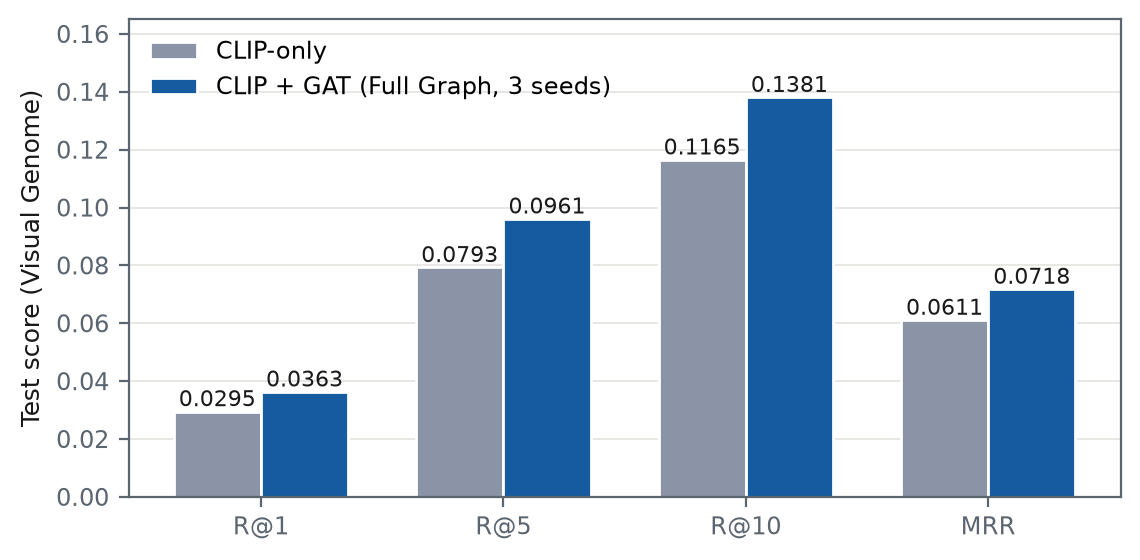
\includegraphics[width=\linewidth]{assets/charts/l1_retrieval.png}
    \end{column}
    \begin{column}{0.42\textwidth}
      \begin{alertblock}{Phát hiện chính}\footnotesize
        Test MRR \textbf{0.0611 $\rightarrow$ 0.0718 $\pm$ 0.0002} (3 seeds), tăng tương đối \textbf{+17.4\%}; R@1 0.0295 $\rightarrow$ 0.0363.
      \end{alertblock}
      \vspace{0.15cm}
      \begin{itemize}\footnotesize
        \item Cùng phép chia tập, cùng CLIP đóng băng, chỉ khác biệt ở bước xếp hạng lại bằng đồ thị.
        \item Độ lệch chuẩn (SD) giữa các seed rất nhỏ $=$ ổn định dưới giao thức này (không suy rộng sang cross-domain).
        \item Mức tăng bị chặn trên bởi không gian ứng viên top-50.
      \end{itemize}
      \vspace{0.15cm}
      {\footnotesize\color{Slate} Bằng chứng: Báo cáo Bảng VII (tập test, Visual Genome, 3 seeds).}
    \end{column}
  \end{columns}
\end{frame}

% ===========================================================================
% 07 --- Level 1 interpretation
% ===========================================================================
\begin{frame}{\leveltag{L1Blue}{CẤP ĐỘ 1} Phần lớn Mức tăng Vẫn Duy trì Dù Thiếu Cạnh Thật}
  \begin{columns}[t]
    \begin{column}{0.50\textwidth}
      \centering
      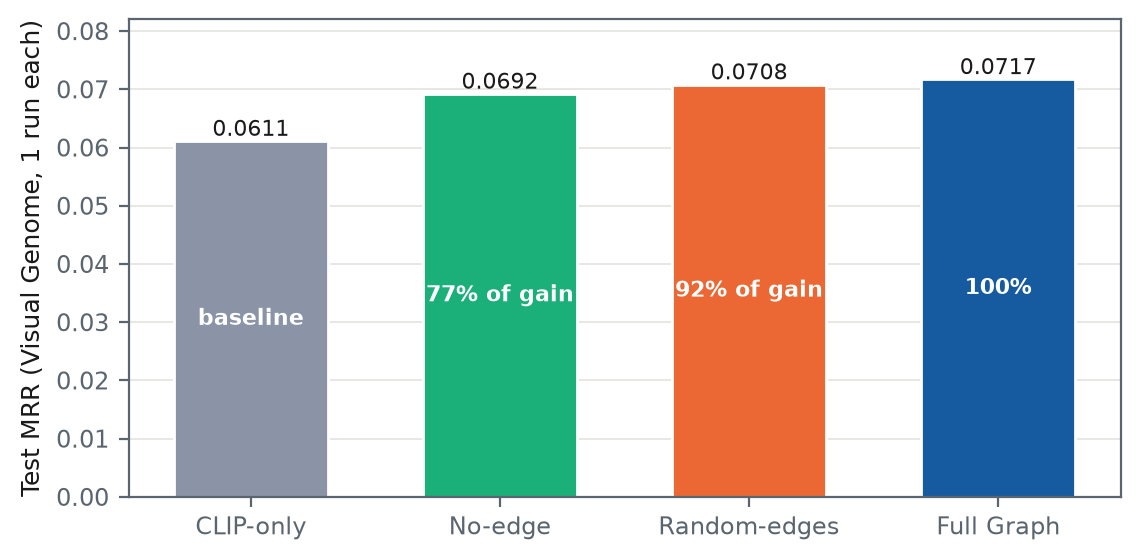
\includegraphics[width=0.86\linewidth]{assets/charts/l1_ablation.png}\\[0.02cm]
      {\footnotesize\color{Slate} Bảng VIII --- 1 lần chạy mỗi cấu hình, cùng khởi tạo.}\\[0.08cm]
      \begin{alertblock}{Nhận định trung thực}\footnotesize
        Trên Visual Genome, mức tăng chủ yếu đến từ \textbf{phép biến đổi đặc trưng học được}, không phải cấu trúc quan hệ --- một phần dư \textbf{nhỏ, trên 1 lần chạy}.
      \end{alertblock}
    \end{column}
    \begin{column}{0.48\textwidth}
      \begin{itemize}\footnotesize
        \item \textbf{No-edge} (phép chiếu học được, không truyền tin) giữ được \textbf{77\%} mức tăng; \textbf{random-edges} giữ \textbf{92\%}.
        \item Đồ thị đầy đủ chỉ vượt random-edges khoảng ${\approx}0.0009$ MRR (1 lần chạy).
        \item Phân tích giải thích đồng thuận: \textbf{75\%} phần tử được giải thích là cạnh \texttt{contains}; quan hệ vật thể--vật thể đóng góp rất ít.
        \item Ca ``peace sign'': hạng CLIP 15 $\rightarrow$ 1; khi loại bỏ tập giải thích thì tụt về hạng 4.
      \end{itemize}
    \end{column}
  \end{columns}
\end{frame}
% ===========================================================================
% 08 --- Level 2 methodology
% ===========================================================================
\begin{frame}{\leveltag{L2Orange}{CẤP ĐỘ 2} MMKG Bổ sung Quan hệ Vượt ra Ngoài Ảnh Cục bộ}
  \begin{columns}[c]
    \begin{column}{0.50\textwidth}
      \begin{block}{Khái niệm: Truy vấn Gián tiếp (Indirect)}\scriptsize
        Không nêu thực thể đích; cho neo và quan hệ để tìm đầu hoặc đuôi bộ ba.\\
        \textit{Ví dụ: ``Người chịu ảnh hưởng bởi Richard Dawkins'' $\rightarrow$ Hitchens.}\\
        (CLIP thuần còn hạn chế ở nhóm truy vấn gián tiếp).
      \end{block}
      \vspace{0.06cm}
      \begin{itemize}\scriptsize
        \item Đồ thị Cấp 1 là từng ảnh riêng lẻ --- MMKG kết nối tri thức toàn cục.
        \item Thực thể $=$ \textbf{cấu trúc + văn bản + thị giác} (AdaMF attention).
        \item Chấm điểm bộ ba bằng \textbf{RotatE}; tắt MAT đối nghịch ($\mu=0$).
      \end{itemize}
      \vspace{0.04cm}
      \begin{center}
      \resizebox{0.92\linewidth}{!}{%
      \begin{tikzpicture}[
        m/.style={draw=LineGray, fill=SoftBg, rounded corners=2pt, font=\scriptsize,
                  align=center, inner sep=3pt, minimum height=0.55cm},
        ar/.style={-{Latex[length=2mm]}, Slate}
      ]
        \node[m] (t) {đ.trưng\\text};
        \node[m, right=0.25cm of t] (v) {đ.trưng\\ảnh};
        \node[m, right=0.25cm of v] (s) {embedding\\cấu trúc};
        \node[m, fill=L2Orange, text=white, right=0.45cm of s] (f) {kết hợp\\AdaMF};
        \node[m, right=0.25cm of f] (r) {điểm số\\RotatE};
        \draw[ar] (t) -- (f); \draw[ar] (v) -- (f); \draw[ar] (s) -- (f);
        \draw[ar] (f) -- (r);
      \end{tikzpicture}}
      \end{center}
    \end{column}
    \begin{column}{0.48\textwidth}
      \begin{block}{Tập dữ liệu (chuẩn đề bài)}\scriptsize
        \textbf{DB15K}: 12.842 thực thể, 279 quan hệ, 25.925 ảnh.\\[0.04cm]
        \textbf{FB15K-237-IMG}: 14.541 thực thể, 237 quan hệ, 139.814 ảnh.
      \end{block}
      \vspace{0.06cm}
      \begin{block}{Nhóm truy vấn kiểm thử}\scriptsize
        \textbf{Trực tiếp (Direct)}: Cho tên thực thể (CLIP đã rất mạnh).\\
        \textbf{Gián tiếp (Indirect)}: 3.195 (DB15K) và 24.564 (FB15K) truy vấn.
      \end{block}
      \vspace{0.06cm}
      {\scriptsize\color{Slate} Cài đặt từ AdaMF-MAT (LREC-COLING 2024), điều chỉnh cho truy hồi ảnh.}
    \end{column}
  \end{columns}
\end{frame}
% ===========================================================================
% 09 --- Level 2 results
% ===========================================================================
\begin{frame}{\leveltag{L2Orange}{CẤP ĐỘ 2} Truy vấn Gián tiếp Dẫn dắt Mức tăng trên Cả Hai MMKG}
  \begin{columns}[c]
    \begin{column}{0.56\textwidth}
      \centering
      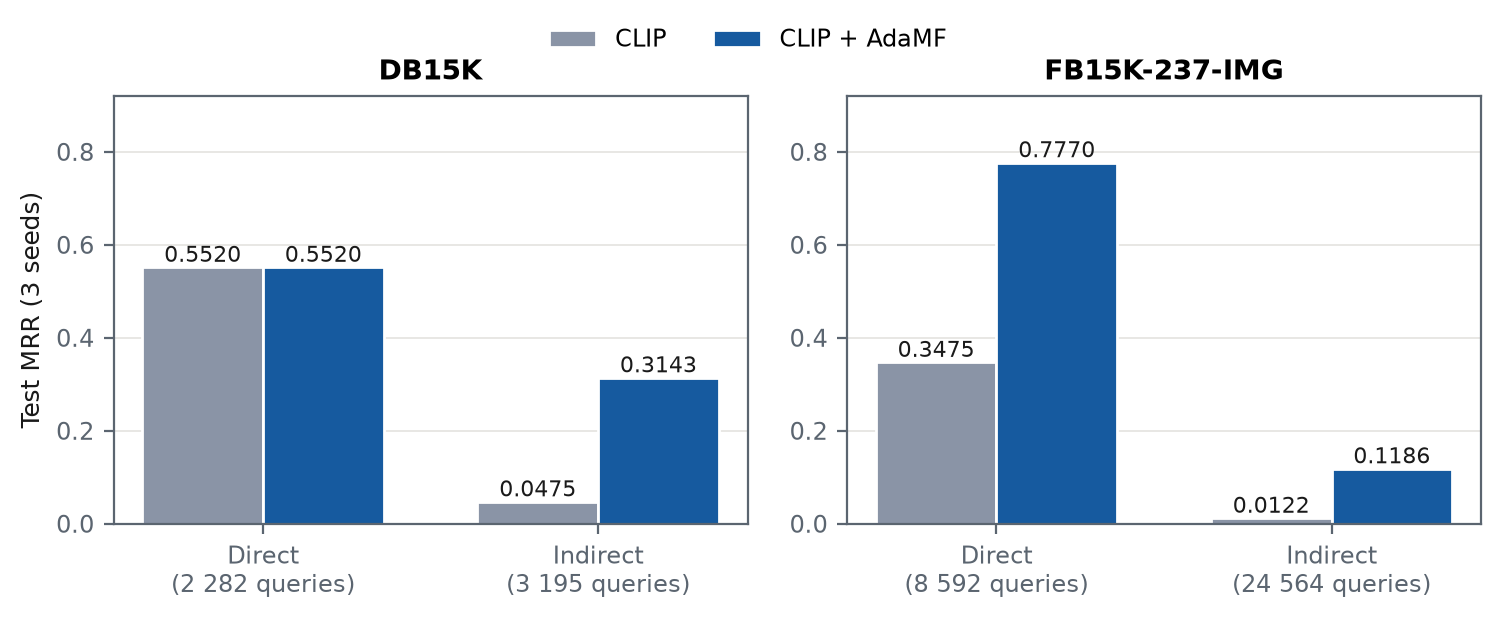
\includegraphics[width=\linewidth]{assets/charts/l2_direct_indirect.png}
    \end{column}
    \begin{column}{0.42\textwidth}
      \begin{alertblock}{Điểm nhấn bứt phá}\footnotesize
        MRR gián tiếp: DB15K \textbf{0.0475 $\rightarrow$ 0.3143} ($6.6\times$); FB15K \textbf{0.0122 $\rightarrow$ 0.1186} ($9.7\times$).
      \end{alertblock}
      \vspace{0.06cm}
      \begin{itemize}\footnotesize
        \item \textbf{Truy vấn gián tiếp}: MRR đạt tới $\mathbf{9.7\times}$ mức CLIP trong giao thức đã xét.
        \item \textbf{Truy vấn trực tiếp}: Giữ nguyên 0.5520 trên DB15K \textbf{theo thiết kế} (bảo toàn ưu thế CLIP).
        \item \textbf{GAT vs AdaMF}: Chưa phát hiện khác biệt có ý nghĩa thống kê trên DB15K (0.3110 so với 0.3143; CI chứa 0).
        \item Độ lệch chuẩn $\le 0.003$ qua 3 seeds (rất ổn định).
      \end{itemize}
      \vspace{0.05cm}
      {\scriptsize\color{Slate} Bảng X. Không so sánh chéo MRR giữa các tập dữ liệu.}
    \end{column}
  \end{columns}
\end{frame}
% ===========================================================================
% 10 --- Level 2 ablation
% ===========================================================================
\begin{frame}{\leveltag{L2Orange}{CẤP ĐỘ 2} Phá Cạnh Làm Giảm Lợi ích Nhiều hơn trên DB15K}
  \begin{columns}[c]
    \begin{column}{0.54\textwidth}
      \centering
      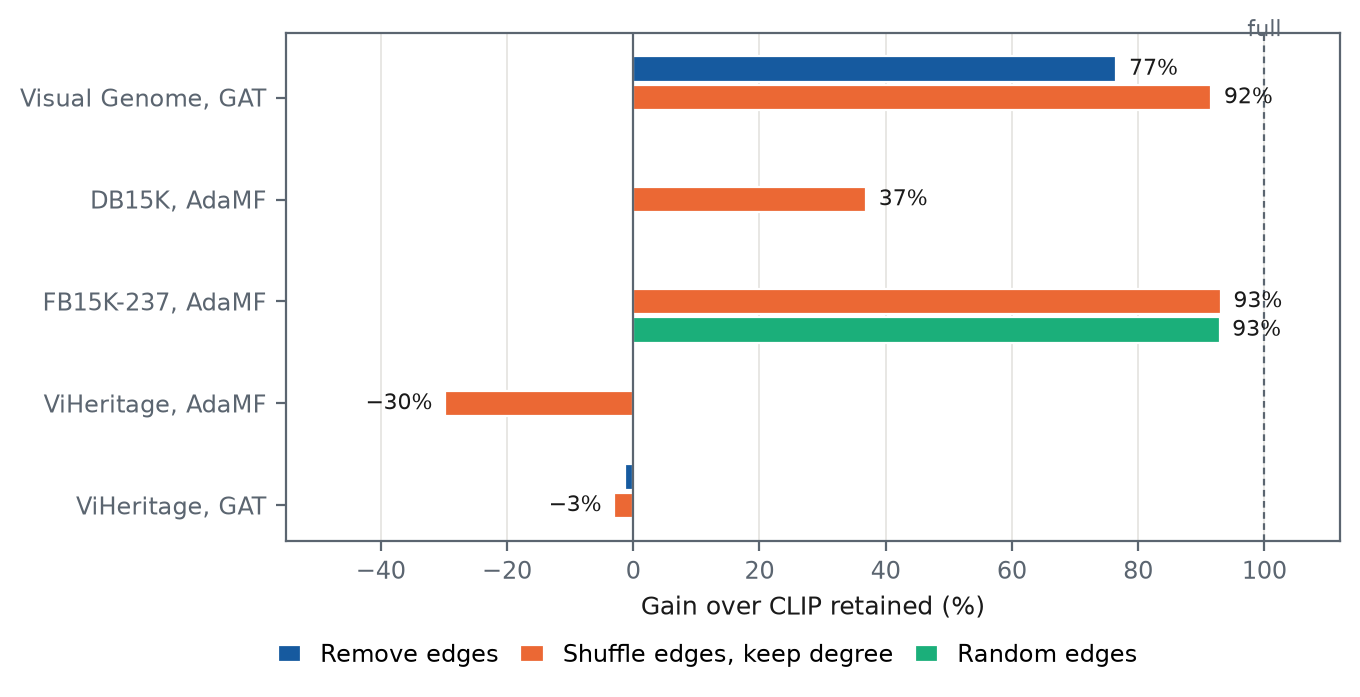
\includegraphics[width=\linewidth]{assets/charts/gain_kept.png}\\[0.05cm]
      {\scriptsize\color{Slate} Phần lợi ích MRR gián tiếp vượt CLIP còn giữ lại (1 lần chạy mỗi cấu hình).}
    \end{column}
    \begin{column}{0.44\textwidth}
      \begin{alertblock}{Diễn giải từ đối chứng}\footnotesize
        \textbf{DB15K}: Xáo cạnh chỉ giữ khoảng 37\% lợi ích, hỗ trợ đóng góp của quan hệ đúng.\\[0.04cm]
        \textbf{FB15K}: Phần lớn lợi ích còn tồn tại sau can thiệp; chưa cô lập được đóng góp riêng của quan hệ.
      \end{alertblock}
      \vspace{0.06cm}
      \begin{itemize}\scriptsize
        \item \textbf{DB15K}: No Edges bỏ huấn luyện, đặt $\alpha=1$; Random Graph được validation chọn $\alpha=1$.
        \item \textbf{FB15K}: No Edges về CLIP (giữ 0\% lợi ích); xáo cạnh và ngẫu nhiên giữ khoảng 93\%.
        \item Ảnh/thực thể: FB15K $\approx9.62$, DB15K $\approx2.02$ (gấp 4.76 lần); chưa chứng minh mật độ ảnh gây học tắt.
      \end{itemize}
      \vspace{0.04cm}
      {\scriptsize\color{Slate} Báo cáo Bảng XI. Tỷ lệ giữ lại tính trên phần tăng so với CLIP, không phải MRR tổng.}
    \end{column}
  \end{columns}
\end{frame}
% ===========================================================================
% 11 --- Level 3 method
% ===========================================================================
\begin{frame}{\leveltag{L3Aqua}{CẤP ĐỘ 3} Giải thích bằng Can thiệp lên Hàm Xếp hạng}
  \begin{center}
  \begin{tikzpicture}[
    n/.style={draw=LineGray,fill=SoftBg,rounded corners=3pt,align=center,font=\footnotesize,minimum width=3.9cm,minimum height=0.85cm},
    ar/.style={-{Latex[length=2.5mm]},L3Aqua,thick}]
    \node[n] (a) {Ảnh hạng 1 của mô hình};
    \node[n,right=0.65cm of a] (b) {Xóa / che / học lại\\để đo ảnh hưởng của bằng chứng};
    \node[n,right=0.65cm of b] (c) {Chấm lại và so với\\bỏ cùng số phần tử ngẫu nhiên};
    \draw[ar] (a)--(b); \draw[ar] (b)--(c);
  \end{tikzpicture}
  \end{center}
  \vspace{0.05cm}
  \begin{columns}[t]
    \begin{column}{0.48\textwidth}
      \begin{block}{Can thiệp sau huấn luyện (post-hoc)}\footnotesize
        \begin{itemize}
          \item \textbf{GAT}: che quan hệ, tính lại bằng checkpoint gốc.
          \item \textbf{AdaMF}: xấp xỉ bằng học lại nhúng cấu trúc cục bộ; giữ các tham số khác cố định.
          \item Chọn tối đa $K^\star$ phần tử có đóng góp dương; $K^\star$ chọn trên validation.
        \end{itemize}
      \end{block}
    \end{column}
    \begin{column}{0.50\textwidth}
      \begin{block}{Các thước đo}\footnotesize
        $\mathrm{Fid}^{+}=(p_0-p_{-S})/p_0$: bỏ tập $S$.\\[0.04cm]
        $\mathrm{Fid}^{-}=(p_0-p_S)/p_0$: chỉ giữ $S$.\\[0.04cm]
        $p$: xác suất softmax từ điểm dung hợp.\\[0.04cm]
        \textbf{PN/PS}: mất / giữ top-1 sau can thiệp.\\
        \textbf{Sparsity}: tỷ lệ phần tử bị lược bỏ.\\
        \textbf{Validity cấu trúc}: bằng chứng hợp lệ trong đồ thị.
      \end{block}
    \end{column}
  \end{columns}
  \vspace{0.08cm}
  {\scriptsize\color{Slate} Mẫu đánh giá: VG 500 truy vấn; DB15K và FB15K 70 truy vấn mỗi tập; ViHeritage 54 với GAT, 50 với AdaMF (không cộng thành 104 truy vấn duy nhất).}
\end{frame}

% ===========================================================================
% 12 --- Level 3 XAI evaluation
% ===========================================================================
\begin{frame}{\leveltag{L3Aqua}{CẤP ĐỘ 3} XAI: Tác động vượt Đối chứng Ngẫu nhiên}
  \begin{columns}[c]
    \begin{column}{0.56\textwidth}
      \centering
      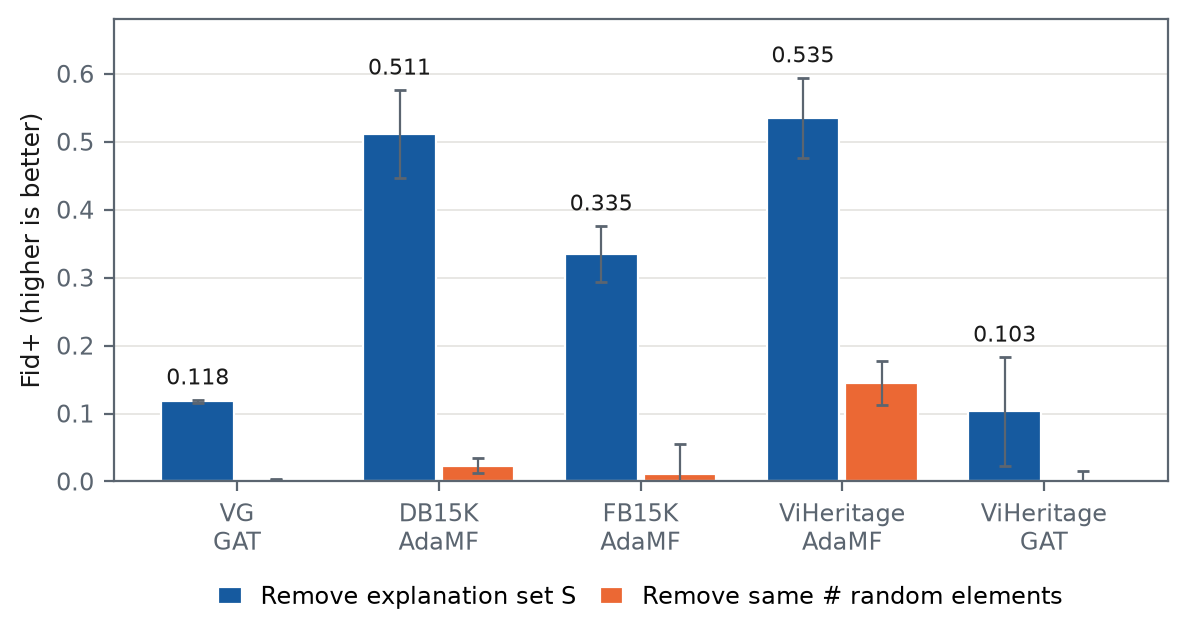
\includegraphics[width=\linewidth]{assets/charts/xai_fidelity.png}
    \end{column}
    \begin{column}{0.42\textwidth}
      \begin{itemize}\footnotesize
        \item \textbf{Trung bình trên 5 cặp mô hình/dữ liệu}: bỏ $S$ làm giảm xác suất softmax nhiều hơn bỏ ngẫu nhiên cùng số phần tử.
        \item \textbf{Validity cấu trúc: 100\%} trong mẫu; không đồng nghĩa đúng ngữ nghĩa. Sparsity tại $K^\star$ khoảng 0.65--0.80, tùy tập nền.
        \item \textbf{Huấn luyện lại AdaMF ViHeritage}: Fid+ 0.327 so với 0.180 ngẫu nhiên ($p=0.0002$).
      \end{itemize}
      \begin{alertblock}{Giới hạn của phép xấp xỉ}\footnotesize
        Spearman(Fid+ xấp xỉ, huấn luyện lại) $=0.32$: mức phù hợp theo từng truy vấn còn hạn chế. Fidelity không xác nhận tính đúng theo kiến thức thực tế.
      \end{alertblock}
    \end{column}
  \end{columns}
\end{frame}
% ===========================================================================
% 13 --- Vietnamese MMKG
% ===========================================================================
\begin{frame}{\leveltag{L3Aqua}{CẤP ĐỘ 3} ViHeritage-MMKG: Di sản Việt Nam}
  \begin{columns}[c]
    \begin{column}{0.39\textwidth}
      \begin{block}{Dữ liệu tự xây}\footnotesize
        \textbf{Miền}: di sản và danh thắng Việt Nam.\\[0.10cm]
        \begin{tabularx}{\linewidth}{@{}L{2.65cm}X@{}}
          Thực thể (có ảnh) & 150 (88)\\[0.04cm]
          Quan hệ / bộ ba & 15 / 427\\[0.04cm]
          Bộ ba train/val/test & 318 / 53 / 56\\[0.04cm]
          Ảnh train/val/test & 264 / 86 / 88\\[0.04cm]
          Truy vấn test & 88 trực tiếp; 54 gián tiếp\\[0.04cm]
          Bộ ba suy ra & Khoảng 35\%\\
        \end{tabularx}
      \end{block}
      {\scriptsize\color{Slate} Kiểm tra liên kết ảnh: 0.935 trên mẫu 100 ảnh, có hỗ trợ AI; chưa có chấm độc lập nhiều người. Nguồn: Wikidata, Wikipedia, Commons; giấy phép ghi trong Data Card.}
    \end{column}
    \begin{column}{0.59\textwidth}
      \centering
      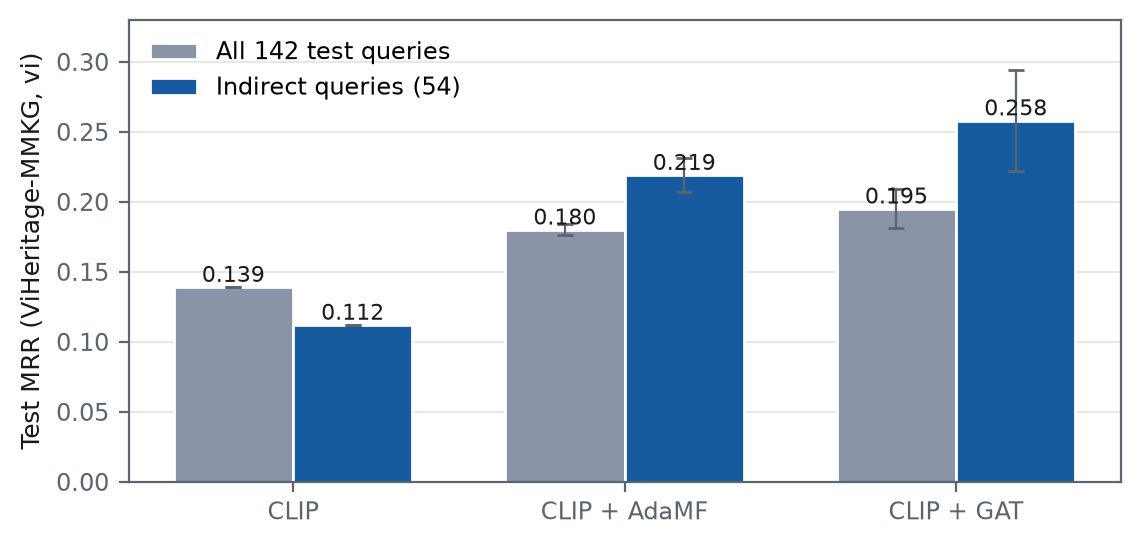
\includegraphics[width=0.94\linewidth]{assets/charts/viheritage.png}
      \vspace{-0.08cm}
      \begin{exampleblock}{MRR gián tiếp: $0.112\to0.219$ / $0.258$}\footnotesize
        AdaMF / GAT, 3 seed; truy vấn tiếng Việt. Ca Huế: Chùa Thiên Mụ được đưa lên hạng 1.
      \end{exampleblock}
      \begin{itemize}\scriptsize
        \item \textbf{Che văn bản}: MRR 0.230; chưa thấy suy giảm so với bản đầy đủ.
        \item \textbf{Xáo cạnh}: MRR thấp hơn CLIP ở các lượt chạy đã xét.
      \end{itemize}
    \end{column}
  \end{columns}
\end{frame}

% ===========================================================================
% 14 --- Cross-level findings
% ===========================================================================
\begin{frame}{Những Gì Thực nghiệm Hỗ trợ --- và Chưa Thể Khẳng định}
  \begin{columns}[t]
    \begin{column}{0.48\textwidth}
      \begin{block}{\textcolor{white}{Được hỗ trợ bởi thực nghiệm}}\footnotesize
        \begin{itemize}
          \item Xếp hạng tăng cường đồ thị vượt CLIP trên mọi tập dữ liệu thử nghiệm (3 seeds cho mô hình đầy đủ).
          \item Mức tăng lớn nhất, ổn định nhất ở truy vấn \textbf{gián tiếp} ($6.6\times$ / $9.7\times$ / ${\approx}2\times$).
          \item Đối chứng hỗ trợ đóng góp của \textbf{quan hệ đúng} trên \textbf{DB15K} và \textbf{ViHeritage} trong giao thức đã xét.
          \item Bằng chứng \textbf{nhạy với can thiệp}: Fid+ vượt ngẫu nhiên ở mức trung bình; validity cấu trúc 100\% trong mẫu.
        \end{itemize}
      \end{block}
    \end{column}
    \begin{column}{0.48\textwidth}
      \begin{alertblock}{\textcolor{white}{Không khẳng định / Vấn đề mở}}\footnotesize
        \begin{itemize}
          \item Trên \textbf{Visual Genome}, phần lớn mức tăng vẫn tồn tại khi xóa cạnh --- cấu trúc quan hệ chỉ là phần dư nhỏ (1 seed).
          \item Trên \textbf{FB15K-237-IMG}, đồ thị nhiễu vẫn giữ ${\approx}93\%$ --- mức tăng không thể quy kết cho quan hệ.
          \item AdaMF và GAT trên DB15K: \textbf{chưa phát hiện khác biệt có ý nghĩa thống kê} (CI chứa 0).
          \item Fidelity $\ne$ chân lý thế giới thực; ablation 1 lần chạy; trần top-50; không so sánh chéo MRR giữa các tập.
        \end{itemize}
      \end{alertblock}
    \end{column}
  \end{columns}
  \vspace{0.1cm}
  \begin{center}
    \footnotesize\itshape\color{Slate}
    ``Đồ thị giúp ích tại những nơi truy vấn đòi hỏi suy luận trên các quan hệ.'' --- Báo cáo Mục VII
  \end{center}
\end{frame}
% ===========================================================================
% 15 --- Conclusions & demo
% ===========================================================================
\begin{frame}{Kết luận \& Kế hoạch Live Demo}
  \begin{columns}[t]
    \begin{column}{0.55\textwidth}
      \begin{block}{3 Thông điệp kết luận cốt lõi}\footnotesize
        \begin{enumerate}
          \item \textbf{Truy hồi (Retrieval)}: GAT nâng MRR Visual Genome $+17.4\%$ (3 seeds) --- lưu ý: phần lớn đến từ đặc trưng vật thể.
          \item \textbf{Tri thức (Knowledge)}: MMKG nâng MRR truy vấn gián tiếp lên tới $\mathbf{9.7\times}$ --- đối chứng hỗ trợ đóng góp của quan hệ đúng trên DB15K.
          \item \textbf{Giải thích (XAI)}: Bằng chứng nhạy với can thiệp; validity cấu trúc 100\% trong mẫu, chưa bảo đảm đúng ngữ nghĩa.
        \end{enumerate}
      \end{block}
      \vspace{0.04cm}
      \begin{block}{Giới hạn nêu rõ từ đầu}\scriptsize
        ablation 1 seed $\cdot$ chưa cô lập cấu trúc trên FB15K $\cdot$ fidelity $\ne$ chân lý thực tế $\cdot$ kiểm tra có AI hỗ trợ chưa có đồng thuận đa chuyên gia.
      \end{block}
    \end{column}
    \begin{column}{0.43\textwidth}
      \begin{block}{\textcolor{white}{Kế hoạch Demo (4--5 phút)}}\footnotesize
        \begin{enumerate}
          \item \textbf{L1}: text query $\rightarrow$ CLIP top-5 $\rightarrow$ GAT rerank.
          \item \textbf{L2}: direct vs indirect query trên DB15K.
          \item \textbf{L3}: can thiệp xóa-$S$ vs xóa ngẫu nhiên.
          \item \textbf{ViHeritage}: truy vấn tiếng Việt + Data Card.
        \end{enumerate}
      \end{block}
      \vspace{0.04cm}
      \begin{exampleblock}{Phương án dự phòng}\scriptsize
        Video quay sẵn $\le$ 5 phút (quy định Mục 8) + checkpoint nạp sẵn nếu có sự cố.
      \end{exampleblock}
      \vspace{0.04cm}
      \begin{center}
        \small\bfseries\color{HCMUSBlue} Xin chân thành cảm ơn Quý Thầy Cô!
      \end{center}
    \end{column}
  \end{columns}
\end{frame}

% ===========================================================================
% BACKUP SLIDES (Appendix)
% ===========================================================================
\appendix
\backupslidestrue

% ===========================================================================
% BACKUP 1 --- metrics & protocol
% ===========================================================================
\stepcounter{backupslide}
\begin{frame}[noframenumbering]{B1: Thước đo và Giao thức Đánh giá}
  \begin{columns}[t]
    \begin{column}{0.48\textwidth}
      \begin{block}{Thước đo truy hồi}\footnotesize
        \textbf{Recall@K}: tỷ lệ truy vấn có ít nhất 1 ảnh phù hợp trong top-$K$.\\[0.1cm]
        \textbf{MRR}: mean reciprocal rank của ảnh phù hợp tốt nhất; xếp hạng lạc quan (optimistic, chỉ đếm điểm thực sự lớn hơn).\\[0.1cm]
        \textbf{MRR Trực tiếp / Gián tiếp}: tính riêng cho từng nhóm truy vấn (quy định Mục 7 đề bài).
      \end{block}
      \vspace{0.15cm}
      \begin{block}{Seeds \& Lựa chọn mô hình}\footnotesize
        3 seeds cho mô hình đầy đủ (trung bình $\pm$ độ lệch chuẩn mẫu, $n{-}1$); ablation chạy 1 lần (nêu rõ). $\alpha$, checkpoint, $K^\star$ --- chỉ chọn trên validation; test chỉ đánh giá đúng 1 lần.
      \end{block}
    \end{column}
    \begin{column}{0.50\textwidth}
      \begin{block}{Kiểm soát rò rỉ dữ liệu}\footnotesize
        \begin{itemize}
          \item VG: gom cụm SHA-256 + pHash \emph{trước khi} phân chia --- các ảnh gần trùng ở cùng một tập.
          \item DB15K: loại bỏ validation chính thức (2.423 dòng trùng lặp); chia lại sạch 90/10 (seed 2027); test chính thức đồng nhất từng byte.
          \item FB15K: cụm ảnh được băm trước khi chia (seed 2026); loại bỏ trùng lặp xuyên thực thể.
          \item Đặc trưng thị giác thực thể chỉ lấy trung bình từ ảnh tập \emph{train}.
          \item Can thiệp tráo cạnh loại trừ va chạm val/test (công bố rõ, không mù hoàn toàn).
          \item ViHeritage: kiểm tra che văn bản chống rò rỉ tên (38.9\% truy vấn gián tiếp chứa tên thực thể neo).
        \end{itemize}
      \end{block}
    \end{column}
  \end{columns}
\end{frame}

% ===========================================================================
% BACKUP 2 --- 20-query set
% ===========================================================================
\stepcounter{backupslide}
\begin{frame}[noframenumbering]{B2: Bộ 20 Truy vấn Đánh giá}
  \begin{columns}[t]
    \begin{column}{0.50\textwidth}
      \begin{block}{Thiết kế (cố định trước khi xem kết quả)}\footnotesize
        Mỗi tập: 10 trực tiếp + 10 gián tiếp (5 head, 5 tail) từ tập test; loại bỏ truy vấn có thực thể đích không xuất hiện trong train; mỗi thực thể đích tối đa 1 truy vấn; seed cố định.
      \end{block}
      \vspace{0.15cm}
      \begin{block}{Mục đích sử dụng}\footnotesize
        Chỉ phục vụ đánh giá và minh họa giải thích --- \textbf{tuyệt đối không} dùng để tinh chỉnh mô hình (quy định Mục 6 đề bài).
      \end{block}
      \vspace{0.15cm}
      {\footnotesize Ví dụ truy vấn gián tiếp: ``an image of the entity that is related to Angelina Jolie by spouse''.}
    \end{column}
    \begin{column}{0.48\textwidth}
      \begin{block}{Kết quả (Bảng XII)}\footnotesize
        \centering
        \begin{tabular}{@{}lcc@{}}
          \toprule
          Nhóm ($n$) & CLIP & CLIP+AdaMF\\
          \midrule
          DB15K trực tiếp (10) & 0.306 & 0.306\\
          DB15K gián tiếp (10) & 0.003 & \textbf{0.296}\\
          DB15K tất cả (20) & 0.154 & 0.301\\
          \midrule
          FB15K trực tiếp (10) & 0.410 & 0.878\\
          FB15K gián tiếp (10) & 0.012 & 0.025\\
          FB15K tất cả (20) & 0.211 & 0.451\\
          \bottomrule
        \end{tabular}
      \end{block}
      \vspace{0.1cm}
      {\footnotesize\color{Slate} Mẫu 10 truy vấn gián tiếp có độ đại diện hạn chế; Bảng X trên toàn bộ test là bằng chứng hiệu năng chính.}
    \end{column}
  \end{columns}
\end{frame}

% ===========================================================================
% BACKUP 3 --- Case Study 1: Visual Genome
% ===========================================================================
\stepcounter{backupslide}
\begin{frame}[noframenumbering]{B3: Visual Genome --- Ca ``peace sign''}
  \begin{columns}[c]
    \begin{column}{0.65\textwidth}
      \centering
      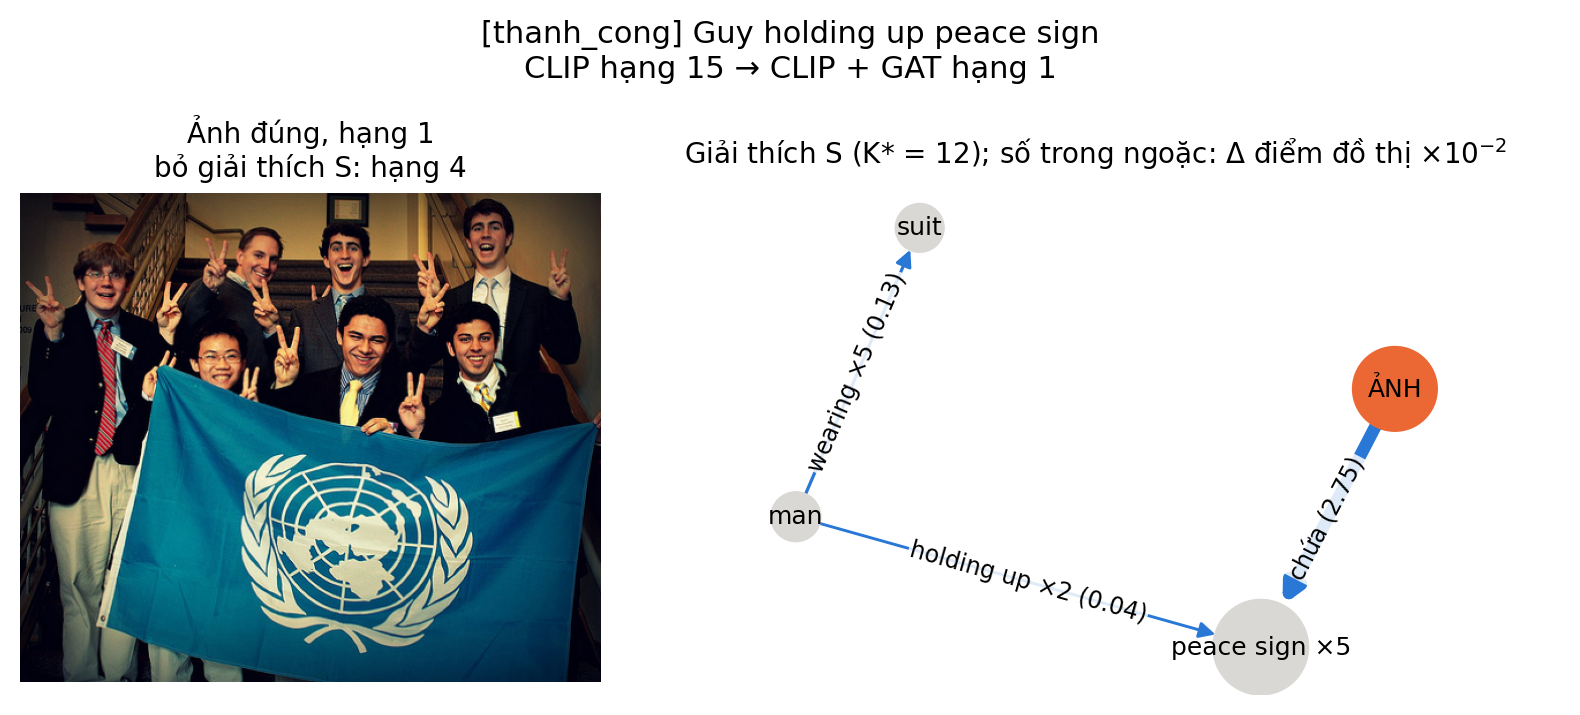
\includegraphics[width=\linewidth]{assets/examples/case_vg_success_peacesign.png}\\[0.05cm]
      {\scriptsize\color{Slate} Cam = nút ảnh; lam = nút vật thể; nhãn cạnh = quan hệ + ($\Delta \times 10^{-2}$).}
    \end{column}
    \begin{column}{0.33\textwidth}
      \begin{block}{\scriptsize Diễn tiến Truy vấn \& Thứ hạng}\scriptsize
        \textbf{Truy vấn}: ``Guy holding up peace sign''\\
        \textbf{Hạng CLIP}: 15\\
        \textbf{Hạng CLIP + GAT}: 1\\
        \textbf{Ablation (xóa $S$)}: tụt về hạng 4\\
        \textbf{No-edge}: 4 \quad \textbf{Random-edges}: 2
      \end{block}
      \vspace{0.1cm}
      \begin{alertblock}{\scriptsize Bóc tách Đóng góp}\scriptsize
        \textbf{Hiện diện vật thể}: \texttt{contains} tới \textit{peace sign} ($\times 5$): $\Delta = 5.5 \times 10^{-2}$ mỗi cạnh.\\
        \textbf{Ràng buộc quan hệ}: \textit{holding up peace sign}: $\Delta = 0.2 \times 10^{-2}$ (nhỏ hơn $27\times$).\\
        $\rightarrow$ Mức tăng rerank đến từ việc khớp vật thể được phát hiện hơn là cạnh quan hệ.
      \end{alertblock}
    \end{column}
  \end{columns}
\end{frame}

% ===========================================================================
% BACKUP 4 --- Case Study 2: DB15K Indirect Query
% ===========================================================================
\stepcounter{backupslide}
\begin{frame}[noframenumbering]{B4: DB15K --- Ca Hitchens và Dawkins}
  \begin{columns}[c]
    \begin{column}{0.65\textwidth}
      \centering
      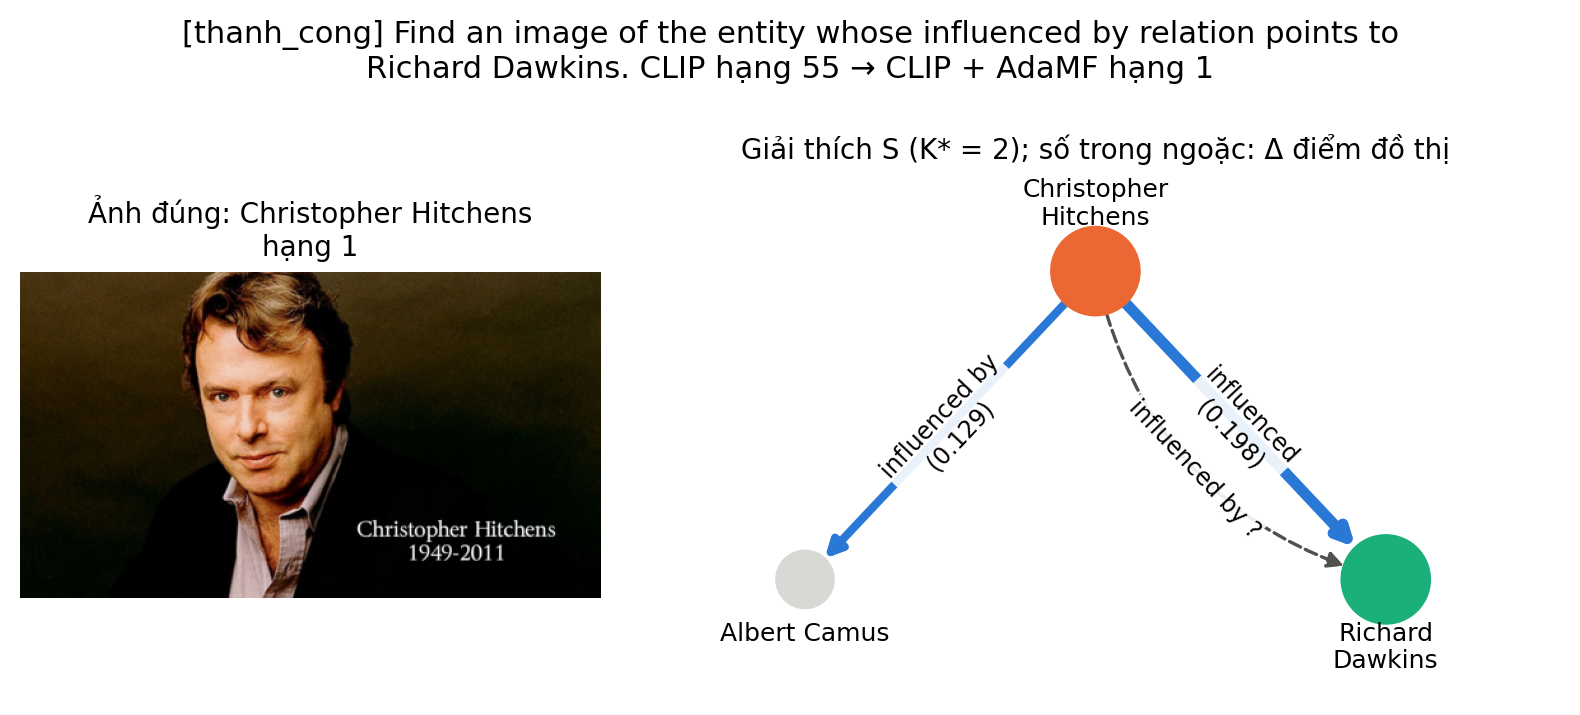
\includegraphics[width=\linewidth]{assets/examples/case_db15k_success_hitchens.png}\\[0.05cm]
      {\scriptsize\color{Slate} Xanh cyan = neo (Dawkins); cam = đích (Hitchens); nét liền = giải thích; nét đứt = truy vấn.}
    \end{column}
    \begin{column}{0.33\textwidth}
      \begin{block}{\scriptsize Diễn tiến Truy vấn \& Thứ hạng}\scriptsize
        \textbf{Truy vấn}: Thực thể chịu ảnh hưởng bởi Dawkins\\
        \textbf{Thực thể đích}: Christopher Hitchens\\
        \textbf{Hạng CLIP}: 55 $\rightarrow$ \textbf{CLIP + AdaMF}: 1 ($K^\star = 2$)
      \end{block}
      \vspace{0.05cm}
      \begin{block}{\scriptsize Che phương thức: mức giảm điểm}\scriptsize
        $\Delta=S_{\text{gốc}}-S_{\text{sau che}}$.\\[0.04cm]
        \textbf{Cấu trúc}: $+74.8$ \quad \textbf{Văn bản}: $+0.20$ \quad \textbf{Ảnh}: $-0.15$\\
        $\rightarrow$ Case này nhạy với che cấu trúc hơn che văn bản hoặc ảnh.
      \end{block}
      \vspace{0.05cm}
      \begin{exampleblock}{\scriptsize Bộ ba Cốt lõi}\scriptsize
        (Hitchens, \textit{influenced}, Dawkins): $\Delta = 0.198$, trực tiếp bắc cầu từ neo sang đích.
      \end{exampleblock}
    \end{column}
  \end{columns}
\end{frame}

% ===========================================================================
% BACKUP 5 --- Case Study 3: ViHeritage Vietnamese MMKG
% ===========================================================================
\stepcounter{backupslide}
\begin{frame}[noframenumbering]{B5: ViHeritage --- Ca Huế và Chùa Thiên Mụ}
  \begin{columns}[c]
    \begin{column}{0.63\textwidth}
      \centering
      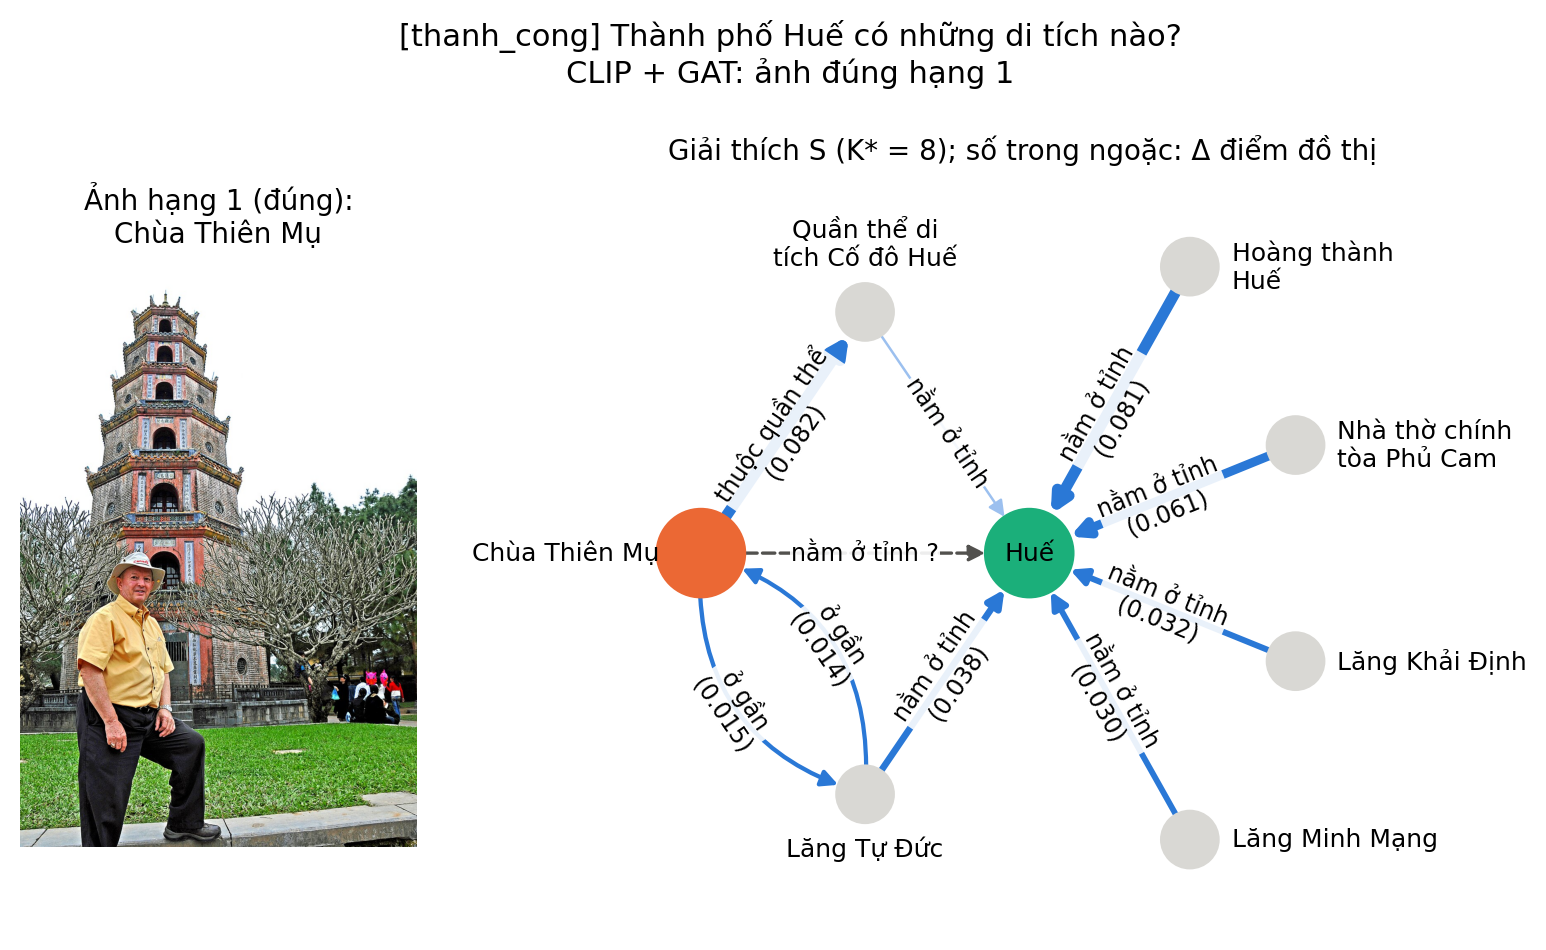
\includegraphics[width=\linewidth]{assets/examples/case_viheritage_gat_hue.png}\\[0.04cm]
      {\scriptsize\color{Slate} Hình 8 báo cáo. Xanh ngọc: Huế; cam: Chùa Thiên Mụ; nét đậm: bằng chứng; nét đứt: quan hệ hỏi.}
    \end{column}
    \begin{column}{0.35\textwidth}
      \begin{block}{\footnotesize Truy vấn và thứ hạng}\scriptsize
        ``Thành phố Huế có những di tích nào?''\\[0.04cm]
        \textbf{Đích}: Chùa Thiên Mụ.\\
        \textbf{CLIP}: 3 $\to$ \textbf{GAT / AdaMF}: 1.
      \end{block}
      \begin{block}{\footnotesize Đường đi hai bước}\scriptsize
        \centering
        \begin{tikzpicture}[
          n/.style={draw=LineGray,fill=SoftBg,rounded corners=2pt,align=center,font=\scriptsize,text width=3.7cm,inner sep=3pt},
          ar/.style={-{Latex[length=1.7mm]},Slate}]
          \node[n] (a) {Chùa Thiên Mụ};
          \node[n,below=0.40cm of a] (b) {Quần thể di tích\\Cố đô Huế};
          \node[n,below=0.40cm of b] (c) {Huế};
          \draw[ar] (a)--node[right,font=\tiny]{thuộc quần thể}(b);
          \draw[ar] (b)--node[right,font=\tiny]{nằm ở tỉnh}(c);
        \end{tikzpicture}
      \end{block}
      \begin{exampleblock}{\footnotesize Can thiệp trên GAT}\scriptsize
        $K^\star=8$; Fid+ 0.49 so với 0.01 ngẫu nhiên.
      \end{exampleblock}
    \end{column}
  \end{columns}
\end{frame}

% ===========================================================================
% BACKUP 6 --- failure cases
% ===========================================================================
\stepcounter{backupslide}
\begin{frame}[noframenumbering]{B6: Phân tích các Ca Thất bại}
  \begin{columns}[t]
    \begin{column}{0.50\textwidth}
      \begin{block}{Cấp độ 1 --- Visual Genome (Bảng IX)}\footnotesize
        \textbf{Thành công (5/5)}: đóng góp hàng đầu luôn là cạnh \texttt{contains} tới vật thể được hỏi; xóa $S$ làm ảnh tụt xuống hạng 2--4.\\[0.08cm]
        \textbf{Thất bại (5)}: 3 ca mà đồ thị \emph{làm giảm hiệu năng} (ảnh sai ở hạng 1 cũng chứa vật thể tương tự --- mô hình tưởng thưởng sự hiện diện thay vì thuộc tính/quan hệ, ví dụ ``black'', ``on the road''); 2 ca không cứu được (hạng 2--5). Trong 3/5 ca, No-edge vẫn xếp ảnh đúng ở hạng 1 --- lỗi xuất hiện khi bổ sung truyền tin (message passing).
      \end{block}
    \end{column}
    \begin{column}{0.48\textwidth}
      \begin{block}{Cấp độ 2 --- DB15K / FB15K}\footnotesize
        \textbf{DB15K thành công}: ảnh đúng tăng từ hạng CLIP 55--624 lên hạng 1; đường đi 1 bước từ neo (ví dụ \texttt{influenced} $\Delta{=}0.198$).\\[0.08cm]
        \textbf{DB15K dạng lỗi}: (i) hai ứng viên cùng chia sẻ quan hệ cận nghĩa với neo; (ii) bộ ba nhiễu làm bằng chứng; (iii) mô hình trả về chính \emph{thực thể neo}.\\[0.08cm]
        \textbf{FB15K thất bại}: thực thể quyết định là nút trung tâm (hub) với hàng nghìn bộ ba; mỗi bộ ba chỉ đóng góp ${\sim}10^{-4}$; che văn bản đôi khi làm tụt điểm nhiều hơn che cấu trúc.
      \end{block}
      \vspace{0.06cm}
      {\footnotesize\color{Slate} Cấp độ 3 (ViHeritage): trả về thực thể neo cho truy vấn dạng ``gần X'' (6/10); bộ ba đúng nhưng không liên quan; lỗi đường dẫn trong Wikidata.}
    \end{column}
  \end{columns}
\end{frame}

% ===========================================================================
% BACKUP 7 --- hyperparameters
% ===========================================================================
\stepcounter{backupslide}
\begin{frame}[noframenumbering]{B7: Cấu hình Huấn luyện}
  \centering\footnotesize
  \resizebox{\textwidth}{!}{%
  \begin{tabular}{@{}l l l l l@{}}
    \toprule
    \textbf{Tham số} & \textbf{VG (GAT)} & \textbf{DB15K (AdaMF)} & \textbf{FB15K-237-IMG} & \textbf{ViHeritage} \\
    \midrule
    Bộ mã hóa đóng băng & CLIP ViT-B/32 (OpenAI) & CLIP ViT-B/32 & CLIP ViT-B/32 & CLIP ViT-B/32; text đa ngữ \\
    Bộ mã hóa đồ thị & GAT 2 lớp nhận biết cạnh, 4$\times$32, dropout 0.2 & AdaMF (struct/text/img), tắt MAT & AdaMF, tắt MAT & AdaMF / GAT 2 lớp \\
    Hàm chấm điểm đồ thị & cosine với nút ảnh & RotatE, dim 250, margin 12 & RotatE, dim 64 & RotatE dim 50/100, margin 6 \\
    Hàm mất mát & CE, 50 hard negatives & self-adversarial sigmoid, 128 neg & CE, 50 hard negatives & sigmoid, 32 negatives \\
    LR / batch & $10^{-4}$ AdamW / 8 truy vấn & $10^{-4}$ / 256 bộ ba & $10^{-4}$ / 8 truy vấn & $5{\times}10^{-4}$ / $2{\times}10^{-3}$, 64 bộ ba \\
    Số epoch tối đa & 100 & 500 & 50 & 1.500 (patience 12) \\
    Tập ứng viên rerank & top-50 CLIP & top-1.000 CLIP & top-1.000 CLIP & toàn bộ 88 ảnh test \\
    $\alpha_{\rm CLIP}$ & 0.6 & 0.0 / 0.1 & 0.1 & 0.0 / 0.1 \\
    \bottomrule
  \end{tabular}}
  \vspace{0.3cm}

  \begin{columns}[t]
    \begin{column}{0.48\textwidth}
      {\footnotesize\color{Slate} Mọi lựa chọn (checkpoint, $\alpha$, cấu hình tối ưu) thực hiện trên validation; test chỉ chạy 1 lần theo cấu hình đã khóa.}
    \end{column}
    \begin{column}{0.48\textwidth}
      {\footnotesize\color{Slate} Thứ tự chạy lại (Phụ lục B báo cáo): Cấp 1 \texttt{run\_gat.py} + ablations + notebook 11; Cấp 2 AdaMF notebooks 07/07b/07c/10a; Cấp 3 notebooks 08a--10d.}
    \end{column}
  \end{columns}
\end{frame}

% ===========================================================================
% BACKUP 8 --- contributions
% ===========================================================================
\stepcounter{backupslide}
\begin{frame}[noframenumbering]{B8: Đóng góp Thành viên và Công bố Công cụ}
  \centering\scriptsize
  \begin{tabularx}{\textwidth}{@{}C{0.6cm}L{4.2cm}Y@{}}
    \toprule
    \textbf{\#} & \textbf{Thành viên} & \textbf{Trách nhiệm chính} \\
    \midrule
    1 & Chung Gia Khánh (23120282) & Thiết kế kiến trúc tổng thể, kiểm định kỹ thuật (audit), ablation, biên tập báo cáo \\
    2 & Lê Hoàng Mỹ Hạ (23120038) & Tiền xử lý dữ liệu, kiểm soát rò rỉ (leakage), trích xuất đặc trưng CLIP \\
    3 & Hàn Vũ Phương Uyên (23120106) & Xây dựng scene graph, cài đặt GAT, phân tích thực nghiệm Cấp độ 1 \\
    4 & Trần Gia Hiển (23120123) & Cài đặt AdaMF trên DB15K \& FB15K-237-IMG, các kiểm soát Cấp độ 2 \\
    5 & Nguyễn An Nghiệp (23127234) & Cơ chế giải thích đồ thị, đánh giá định lượng XAI, xây dựng tập dữ liệu MMKG \\
    \bottomrule
  \end{tabularx}
  \vspace{0.05cm}

  \begin{columns}[t]
    \begin{column}{0.48\textwidth}
      \begin{block}{Danh mục nộp bài}\scriptsize
        Code + môi trường + hướng dẫn $\cdot$ phân chia / seed cố định $\cdot$ báo cáo 18 trang + slide + bảng phân công $\cdot$ notebook truy vấn $\rightarrow$ top-$k$ kèm giải thích $\cdot$ phân tích 5 thành công + 5 thất bại $\cdot$ bộ 20 truy vấn $\cdot$ Data Card ViHeritage $\cdot$ live demo + video $\le$5 phút.
      \end{block}
    \end{column}
    \begin{column}{0.48\textwidth}
      \begin{block}{Khai báo công cụ (Mục 9 đề bài)}\scriptsize
        Mã nguồn mở: AdaMF-MAT (tinh chỉnh), PyTorch Geometric, OpenCLIP, sentence-transformers. Trợ lý AI khai báo trong Phụ lục C của báo cáo (soạn thảo notebook, câu hỏi tiếng Việt, kiểm tra liên kết, rà soát tính hợp lệ, hiệu đính báo cáo) --- nhóm tự kiểm chứng và bảo vệ.
      \end{block}
    \end{column}
  \end{columns}
\end{frame}

\end{document}
